\section{Neighbouring Nodes}\label{sec:neighboring_nodes}
This section starts with a short introduction into Attempto~Controlled~English~(ACE) which is a formal language, capable of expressing domain-specific knowledge by human readable sentences. In the literature~\cite{soton265735} this task is also known under the term \textit{ontology verbalisation}. Even though there exists \textit{OWL~Verbalizer}\footnote{\url{http://mcs.open.ac.uk/nlg/SWAT/Verbaliser.html} accessed 2018/04/30}, a tool which transforms generic ontologies into English sentences, we could not integrate it into the context enrichment process because 
\begin{inparaenum}[1)]
		\item \label{itm:owl_verbalizer_integration_problems_standalone} it was designed as a standalone tool written in SWI-Prolog\footnote{\url{http://www.swi-prolog.org/} accessed 2018/04/30} and
		\item \label{itm:owl_verbalizer_integration_problems_ontology} it only accepts the whole ontology as input
\end{inparaenum}. While~\ref{itm:owl_verbalizer_integration_problems_standalone} could be solved using JPL\footnote{\url{http://www.swi-prolog.org/packages/jpl/} accessed 2018/11/30}, a library written in SWI-Prolog providing a bidirectional interface between Java and Prolog, it is still considered experimental and would require considerable integration efforts. We could not think of a reasonable solution to~\ref{itm:owl_verbalizer_integration_problems_ontology} because crowdsourcing jobs could also be generated from a subset of the concepts defined in an ontology. However, in future versions of OWL~Verbalizer this limitations might be solved as there exists a ticket\footnote{\url{https://github.com/Kaljurand/owl-verbalizer/issues/13} accessed 2018/11/30} for mitigation. 

As in the guidelines for conducting crowdsourcing research~\cite{sarasua2015crowdsourcing}, the authors recommended to avoid technical terms in crowdsourcing questions. In the next paragraphs we explain how \textit{ontology verbalisation} helps to achieve this goal. 

\subsection{Attempto Controlled English (ACE)}
Despite the fact that natural language is desirable for descriptions as everybody knows and understands with no extra learning effort, it conflicts in terms of expressiveness and specificity with well defined ontologies which can encode complex data and relations in domain-specific areas. To resolve this conflict, a new language variant named \textbf{ACE}~\textit{(Attempto Controlled English)}~\cite{fuchs2008} was created. ACE is a formal language, capable of expressing domain-specific knowledge with a well defined syntax, supporting formal reasoning and readable by specialists who are yet unfamiliar with formal languages and methods.

To get a better understanding of ACE\footnote{\url{https://tinyurl.com/yc3zhu9a} accessed 2018/05/05}\footnote{\url{https://tinyurl.com/ycst39jv} accessed 2018/05/05}, a short overview of its language structure is given in the next paragraphs:
 
\paragraph{Simple Sentences} A Simple Sentence derived from standard English language contains a subject, a verb and additional elements: \texttt{subject + verb + complements~[~+~adjuncts~]}. The verb relates directly or indirectly to one or more other objects~(\textit{complements}). Optionally, to add more specificity, one or more adverbs and prepositional phrases can be added~(\textit{adjuncts}). 

\paragraph{Composite Sentences} A Composite Sentence is composed of one or more Simple~Sentences, connected by \textit{coordination},
\textit{subordination}, \textit{quantification} and \textit{negation}. Whereas coordination links sentences either by the word \texttt{and} or \texttt{or}, subordination relates dependent sentences in some way~(e.g. if-then sentences). Quantification allows statements about all~(universal quantification) or certain~(existential quantification) objects of a certain domain. Last, encoding negative polarity in a sentence~(e.g. sentences containing \texttt{not} or \texttt{no}) is defined as negation. 

\paragraph{Query Sentences} Query Sentences can be divided into polar questions~(e.g. with \textit{yes/no} answer) and non-polar questions, also known as \emph{wh-questions}. In contrast to yes/no questions no pre-defined answer exist for these. Furthermore, wh-questions start with either of the following five W-words: \texttt{Who}, \texttt{What}, \texttt{When}, \texttt{Where} and \texttt{Why}. However, this definition somewhat less strict as sometimes questions starting with the word \texttt{How} are included as well.

\paragraph{Anaphoric References} If the meaning of a word or phrase is context dependent, recurring occurrences of these expressions are called \textit{Anaphoric References}. More specifically, the referring term~(\textit{anaphor}) relates to an antecedent expression. For example, given the sentence: \texttt{Tom arrived, but nobody noticed him}, the pronoun \texttt{him} relates to \texttt{Tom}. To resolve ambiguities during the processing phase, Anaphoric References are replaced by encoded references. 

\subsection{Ontology based Approach}\label{sec:enrichment_ontology_approach}
Based on the ACE~rules describes above we implemented an algorithm which generates context descriptions based on subsumption relations. The pseudocode of the overall workflow is given in \hyperref[alg:neighbourhood]{Algorithm~\ref*{alg:neighbourhood}}. The notation to describe properties and relations is based on a formal Ontology~Description Logic~(DL)~\cite{baader2003}, string manipulations were formally defined in~\cite{hopcroft1969}.

\begin{algorithm}
	\caption{Context Enrichment based on Neighbouring Nodes}\label{alg:neighbourhood}
	\begin{algorithmic}[1]
		\Procedure{Generate Description}{}\newline
			\textbf{Input:} A concept $C$\newline
			\textbf{Output:} A textual description $T$ of $C's$ neighbouring nodes based on subsumption\newline
			\State{$T=\{\}$} \label{alg:neighbourhood:text_initialisation}
			\For {$ (c,d) \in C \sqsubseteq D $}
				\State $T=T$ $\cup$ "Every " $\cup$ $name(c)$ $\cup$ " is a " $\cup$ $name(d)$
			\EndFor
			\For {$ (e,c) \in E \sqsubseteq C $}
				\State $T=T$ $\cup$ "Every " $\cup$ $name(e)$ $\cup$ " is a " $\cup$ $name(c)$
			\EndFor
		\EndProcedure
	\end{algorithmic}
\end{algorithm}

The main work is done in two for-loops, which calculate context descriptions based on subsumption~$(\sqsubseteq)$ and string concatenation~$(\cup)$. To handle the case of missing subsumption relations, the output text $T$ is initialised to an empty string~(\hyperref[alg:neighbourhood:text_initialisation]{Line~\ref*{alg:neighbourhood:text_initialisation}}). Next, for every subsumption relation having the input concept $C$ in its signature, either $C's$ name or the anchor node's name is appended first.

A simple ontology graph describing the university domain is given in~\hyperref[fig:simple_owl_graph]{Figure~\ref*{fig:simple_owl_graph}}. It will
be used to illustrate the concept of the context generation algorithm.
\begin{figure}
	 \centering
	 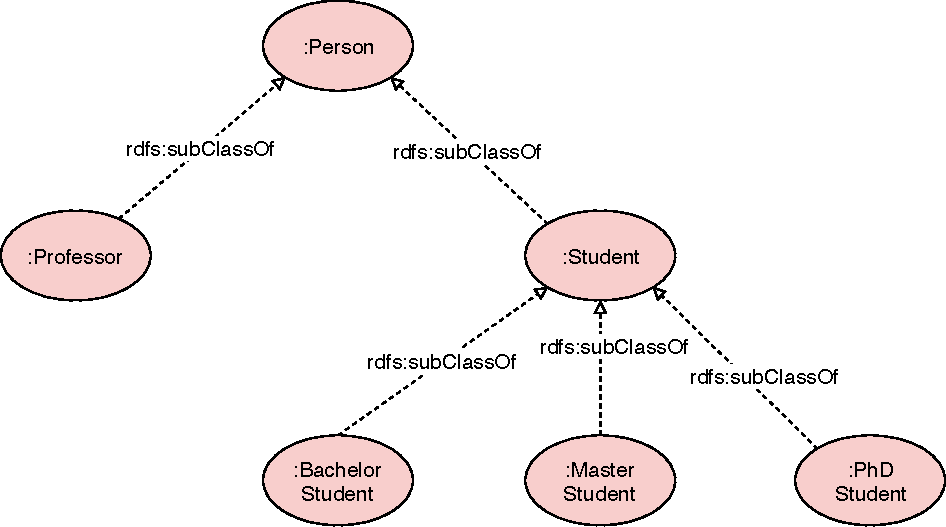
\includegraphics[width=\textwidth]{drawio/University_Ontology_Example-Professor-Student}
	 \caption{Simple Ontology Graph describing the student/professor relationship}\label{fig:simple_owl_graph}
\end{figure}
If the concept \emph{Student} is taken as reference node, the algorithm first collects all subsumption relations having \emph{Student} as child node which gives $\{Person\}$ and generates $T=\{$ \emph{"Every Student is a Person"} $\}$. Next, all subsumption relations having \emph{Student} as parent node were collected which gives $\{$ \emph{Bachelor Student, Master Student, PhD Student} $\}$ and generates $T=\{$ \emph{"Every Student is a Person", "Every Bachelor Student is a Student", "Every Master Student is a Student", "Every PhD Student is a Student"} $\}$. 

After context generation, our platform creates the questionnaire for crowd workers which also includes the actual question for ontology validation and some instructions for guidance. 
\hyperref[fig:university_ontology_questionaire]{Figure~\ref*{fig:university_ontology_questionaire}} depicts the questionnaire presented to crowd workers for the university domain example. 
\begin{figure}
	 \centering
	 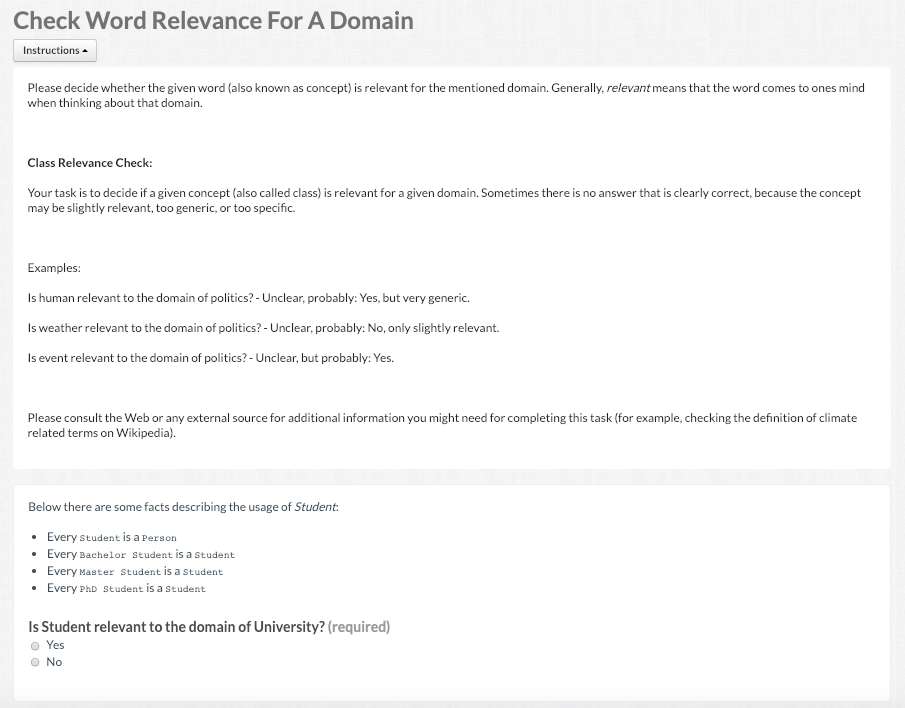
\includegraphics[width=\textwidth]{screenshots/questionaire_university_example}
	 \caption{Questionnaire presented to crowd workers for the university domain example}\label{fig:university_ontology_questionaire}
\end{figure}

